\chapter{网络层:数据平面}

    \emph{在网络中的每一台主机和路由器中都有一个网络层部分。}

    网络层能够被分解为两个相互作用的部分,即数据平面和控制平面。数据平面功能,即网络层中每台路由器的功能,该数据平面功能决定到达路由器输入链路之一的数据报(即网络层的分组)如何转发到该路由器的输出链路之一。我们将涉及传统的IP转发(其中转发基于数据报的目的地址)和通用的转发(其中可以使用数据报首部中的几个不同域的值执行转发和其他功能)。

    网络层的控制平面功能,即网络范围的逻辑,该控制平面功能控制数据报沿着从源主机到目的主机的端到端路径中路由器之间的路由方式。我们将学习路由选择算法,以及广泛用于今天因特网中的诸如OSPF和BGP等路由选择协议。

\section{网络层概述}

    每台路由器的数据平面的主要作用是从其输入链路向其输出链路转发数据报;控制平面的主要作用是协调这些本地的每路由器转发动作,使得数据报沿着源和目的地主机之间的路由器路径最终进行端到端传送。

\subsection{转发和路由选择:数据平面和控制平面}

    网络层的作用从表现上看就是将分组从一台主机发送到另一台主机。

\begin{itemize}
    \item 转发
    \subitem 当一个分组到达路由器的一条输入链路,该路由器必须将该分组移动到适当的输出链路
    \item 路由选择
    \subitem 分组从发送方刘翔接收方,网络层必须决定这些分组采用的路由或路径。计算这些路径的算法被称为路由选择算法(routing algorithm)
\end{itemize}

    此处,给出较为精确的定义:
    
    转发(forwarding)\emph{指将分组从一个输入链路接口转移到适当的输出链路接口的路由器本地动作。转发发生的时间尺度很短。通常用硬件实现}

    路由选择(routing)\emph{指确定分组从源到目的地所采取的端到端路径的网络范围处理过程。路由选择发生的时间尺度长得多。通常用软件实现}

    每台网络路由器中有一个关键元素是它的转发表(forwarding table)。路由器检査到达分组首部的一个或多个字段值,进而使用这些首部值在其转发表中索引,通过这种方法来转发分组。这些值对应存储在转发表项中的值,指出了该分组将被转发的路由器的输出链路接口

\begin{figure}[!htbp]
    \centering
    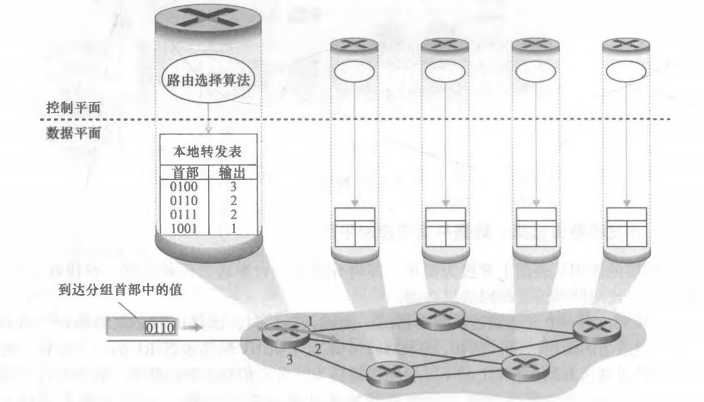
\includegraphics[width=0.8\textwidth]{image/chapter04/路由选择算法.png}
    \caption{路由选择算法决定转发表中的值}
\end{figure}

\subsubsection{控制平面:传统方法}

    路由器中物理上存在的所有转发表的内容是由人类网络操作员直接配置的,进一步说明转发和路由选择功能的区别和不同目的。在这种情况下,不需要任何路由选择协议!当然,这些人类操作员将需要彼此交互,以确保该转发表的配置能使分组到达它们想要到达的目的地。

\subsubsection{控制平面:SDB方法}

    远程控制器计算和分发转发表以供每台路由器所使用。控制平面路由选择功能与物理的路由器是分离的,即路由选择设备仅执行转发,而远程控制器计算并分发转发表。

\begin{figure}[!htbp]
    \centering
    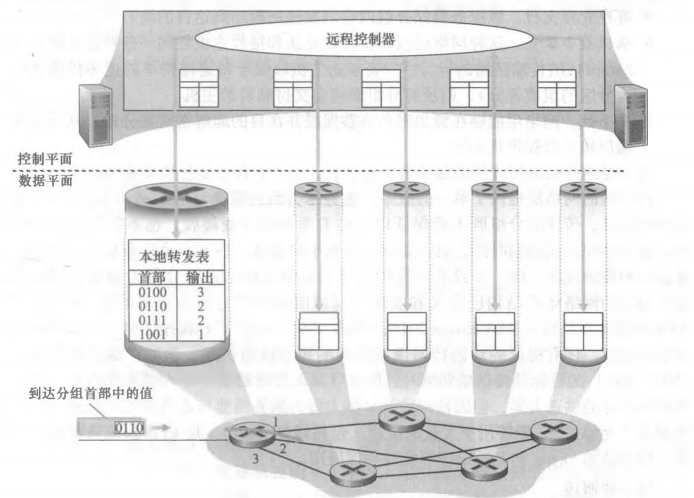
\includegraphics[width=0.6\textwidth]{image/chapter04/远程控制器决定转发表.png}
    \caption{远程控制器确定并分发转发表中的值}
\end{figure}

    显示在图4.2中的控制平面方法是软件定义网络(Software-Defined Networking, SDN)的本质,因为计算转发表并与路由器交互的控制器是用软件实现的,故网络是“软件定义”的。

\subsection{网络服务模型}

    \emph{网络服务模型(network servicemodel)定义了分组在发送与接收端系统之间的端到端运输特性}

    因此,我们考虑网络层能够提供:

\begin{itemize}
    \item 确保交付
    \item 具有时延上界的确保交付
    \item 有序分组交付
    \item 确保最小带宽
    \item 安全性
\end{itemize}

    因特网的网络层提供了单一的服务,称为尽力而为服务(best effort service)。使用尽力而为服务,传送的分组既不能保证以它们发送的顺序被接收,也不能保证它们最终交付;既不能保证端到端时延,也不能保证有最小的带宽。尽力而为服务看起来是根本无服务的一种委婉说法,即一个没有向目的地交付分组的网络也符合尽力而为交付服务的定义!

\section{路由器工作原理}

    我们将注意力转向网络层的转发功能,即实际将分组从一台路由器的入链路传送到适当的出链路

\begin{figure}[!htbp]
    \centering
    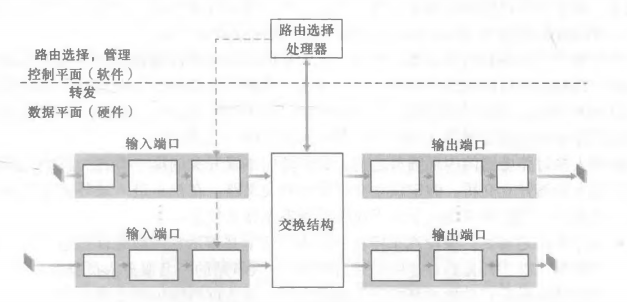
\includegraphics[width=0.8\textwidth]{image/chapter04/路由器体系结构.png}
    \caption{路由器体系结构}
\end{figure}    

\begin{itemize}
    \item 输入端口
    \subitem 在路由器中执行终结入物理链路的物理层功能,位于输入端口最左(输出端口最右)
    \subitem 与入链路远端的数据链路层交互执行数据链路层功能,位于输入输出中间
    \subitem 在输入端执行查找功能,位于输入端口最右,正是这里通过查询转发表决定输出端口
    \item 交换结构 
    \subitem 交换结构将路由器的输入端口连接到输出端口,该结构完全包含在路由器中
    \item 输出端口
    \subitem 输出端口存储从交换结构接收的分组,并通过执行必要的链路层和物理层功能在输出链路上传输这些分组。
    \item 路由选择处理器
    \subitem 路由选择处理器执行控制平面功能。在传统的路由器中,它执行路由选择协议维护路由选择表与关联链路状态信息,并为该路由器计算转发表。
    \subitem 在SDN路由器中,路由选择处理器(在其他活动中)负责与远程控制器通信,目的是接收由远程控制器计算的转发表项,并在该路由器的输入端口安装这些表项。路由选择处理器还执行网络管理功能
\end{itemize}

    路由器的输入端口、输出端口和交换结构几乎总是用硬件实现。

\subsection{输入端口处理和基于目的地转发}

    下图显示了一个更详细的输入处理的视图。

\begin{figure}[!htbp]
    \centering
    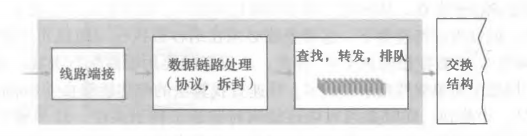
\includegraphics[width=0.6\textwidth]{image/chapter04/输入端口处理.png}
    \caption{输入端口处理}
\end{figure}

    在输入端口中执行的查找对于路由器运行是至关重要的。正是在这个地方,路由器使用转发表来查找输出端口,使得到达的分组能经过交换结构转发到该输出端口。

    转发表是由路由选择处理器计算和更新的(使用路由选择协议与其他网络路由器中的路由选择处理器进行交互),或者转发表接收来自远程SDN控制器的内容。转发表从路由选择处理器经过独立总线(例如一个PCI总线)复制到线路卡

    路由器用分组目的地址的前缀(prefix)与该表中的表项进行匹配;如果存在一个匹配项,则路由器向与该匹配项相关联的链路转发分组。\emph{当有多个匹配时,该路由器使用最长前缀匹配规则(longest prefix matching rule);即在该表中寻找最长的匹配项,并向与最长前缀匹配相关联的链路接口转发分组}

    假定转发表已经存在,从概念上讲表査找是简单的,硬件逻辑只是搜索转发表查找最长前缀匹配。但在G比特速率下,这种查找必须在纳秒级执行。

    因此,不仅必须要用硬件执行查找,而且需要对大型转发表使用超出简单线性搜索的技术;快速查找算法的综述能够在[Gupta 2001, Ruiz Sanchez 2011]中找到。同时必须对内存访问时间给予特别关注,这导致用嵌入式片上DRAM和更快的SRAM (用作一种DRAM缓存)内存来设计。实践中也经常使用三态内容可寻址存储器(Tenary Content Address Memory, TCAM)来查找

    一旦通过查找确定了某分组的输出端口,则该分组就能够发送进入交换结构。在某些设计中,如果来自其他输入端口的分组当前正在使用该交换结构,一个分组可能会在进入交换结构时被暂时阻塞。因此,一个被阻塞的分组必须要在输入端口处排队,并等待稍后被及时调度以通过交换结构

\subsection{交换}

    交换结构位于一台路由器的核心部位, 因为正是通过这种交换结构, 分组才能实际地从一个输入端口交换(即转发)到一个输出端口中。交换可以用许多方式完成

\begin{figure}[!htbp]
    \centering
    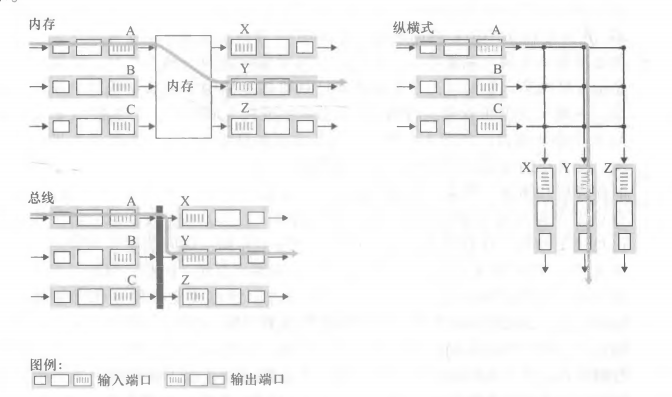
\includegraphics[width=0.6\textwidth]{image/chapter04/三种交换技术.png}
    \caption{三种交换技术}
\end{figure}

\begin{itemize}
    \item 经内存交换
    \subitem 最简单、最早的路由器是传统的计算机,在输入端口与输出端口之间的交换是在CPU(路由选择处理器)的直接控制下完成的。输入与输出端口的功能就像在传统操作系统中的I/O设备一样。
    \subitem 许多现代路由器通过内存进行交换。然而,与早期路由器的一个主要差别是,目的地址的查找和将分组存储(交换)进适当的内存存储位置是由输入线路卡来处理的。在某些方面,经内存交换的路由器看起来很像共享内存的多处理器,用一个线路卡上的处理将分组交换(写)进适当的输出端口的内存中。
    \item 经总线交换
    \subitem 输入端口经一根共享总线将分组直接传送到输出端口,不需要路由选择处理器的干预。
    \subitem 让输入端口为分组预先计划一个交换机内部标签(首部),指示本地输出端口,使分组在总线上传送和传输到输出端口。该分组能由所有输出端口收到,但只有与该标签匹配的端口才能保存该分组。然后标签在输出端口被去除,因为其仅用于交换机内部来跨越总线。
    \item 经互联网络交换
    \subitem 克服单一、共享式总线带宽限制的一种方法是,使用一个更复杂的互联网络。
    \subitem 每条垂直的总线在交叉点与每条水平的总线交叉, 交叉点通过交换结构控制器(其逻辑是交换结构自身的一部分)能够在任何时候开启和闭合。
    \subitem 纵横式交换机是非阻塞的(non-blocking) ,即只要没有其他分组当前被转发到该输出端口,转发到输出端口的分组将不会被到达输出端口的分组阻塞。然而,如果来自两个不同输入端口的两个分组其目的地为根同的输出端口,则一个分组必须在输入端等待,因为在某个时经给定总线仅能发送一个分组
\end{itemize}

\subsection{输出端口处理}

    输出端口处理取出已经存放在输出端口内存中的分组并将其发送到输出链路上。这包括选择和取岀排队的分组进行传输,执行所需的链路层和物理层传输功能

\begin{figure}[!htbp]
    \centering
    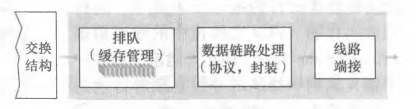
\includegraphics[width=0.8\textwidth]{image/chapter04/输出端口处理.png}
    \caption{输出端口处理}
\end{figure}

\subsection{何处排队}

    在输入端口和输出端口处都可以形成分组队列。排队的位置和程度(或者在输入端口排队,或者在输岀端口排队)将取决于流量负载、交换结构的相对速率和线路速率。

    假定输入线路速度与输出线路速度(传输速率)是相同的,均为$R_{line}$(单位为每秒分组数),并且有N个输入端口和N个输出端口。定义交换结构传送速率$R_{switch}$为从输入端口到输出端口能够移动分组的速率。

\subsubsection{输入排队}

    考虑纵横式交换结构,并假定:
    
\begin{itemize}
    \item [①] 所有链路速度相同;
    \item [②] 一个分组能够以一条输入链路接收一个分组所用的相同的时间量,从任意一个输入端口传送到给定的输出端口
    \item [③] 分组按FCFS方式,从一指定输入队列移动到其要求的输出队列中。
\end{itemize}

    如果位于两个输入队列前端的两个分组是发往同一输出队列的,则其中的一个分组将被阻塞,且必须在输入队列中等待,因为交换结构一次只能传送一个分组到某指定端口。

\begin{figure}[!htbp]
    \centering
    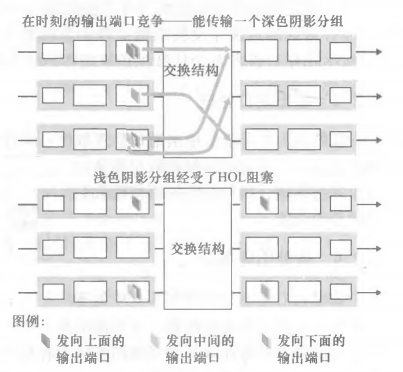
\includegraphics[width=0.6\textwidth]{image/chapter04/输入排队交换机中的HOL阻塞.png}
    \caption{在一个输入排队交换机中的HOL阻塞}
\end{figure}

    左下角队列中的深色阴影分组必须等待。但不仅该分组要等待,左下角队列中排在该分组后面的浅色阴影分组也要等待,即使右中侧输出端口(浅色阴影分组的目的地)中无竞争。

    这种现象叫做输入排毒交换机中的线路前部(Head-Of-the-Line,HOL)阻塞,即在一个输入队列中排队的分组必须等待通过交换结构发送,因为它被位于线路前部的另一个分组阻塞。

\subsubsection{输出排队}

    当没有足够的内存来缓存一个入分组时,就必须做出决定:要么丢弃到达的分组(采用一种称为弃尾(drop tail)的策略),要么删除一个或多个已排队的分组为新来的分组腾出空间。

    在某些情况下,在缓存填满之前便丢弃一个分组(或在其首部加上标记)的做法是有利的,这可以向发送方提供一个拥塞信号。已经提出和分析了许多分组丢弃与标记策略[Labrador 1999, Hollot 2002],这些策略统称为主动队列管理(Active Queue Management ,AQM)算法。随机早期检测(Random Early Detection, RED)算法是得到最广泛研究和实现的AQM算法之一

\begin{figure}[!htbp]
    \centering
    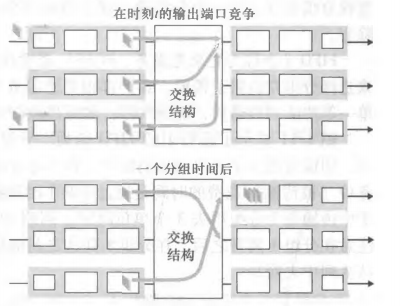
\includegraphics[width=0.6\textwidth]{image/chapter04/输出端口排队.png}
    \caption{输出端口排队}
\end{figure}

    输出端口的分组调度(packet scheduler)在这些排队分组中选择一个分组来传输

\subsection{分组调度}

    现在我们转而讨论确定次序的问题,即排队的分组如何经输出链路传输的问题。

\subsubsection{先进先出}

\begin{figure}[!htbp]
    \centering
    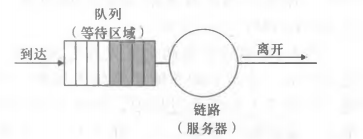
\includegraphics[width=0.6\textwidth]{image/chapter04/FIFO排队抽象.png}
    \caption{FIFO排队抽象}
\end{figure}

    上图显示了对于先进先出(First-In-First-Out, FIFO)链路调度规则的排队模型的抽象。如果链路当前正忙于传输另一个分组,到达链路输出队列的分组要排队等待传输。如果没有足够的缓存空间来容纳到达的分组,队列的分组丢弃策略则确定该分组是否将被丢弃(丢失)或者从队列中去除其他分组以便为到达的分组腾出空间

    FIFO(也称为先来先服务,FCFS)调度规则按照分组到达输出链路队列的相同次序来选择分组在链路上传输。

    下图显示了运行中的FIFO队列。分组的到达由上部时间线上带编号的箭头来指示,用编号指示了分组到达的次序。

\begin{figure}[!htbp]
    \centering
    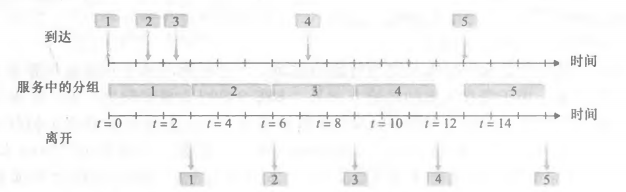
\includegraphics[width=0.6\textwidth]{image/chapter04/运行中的FIFO队列.png}
    \caption{运行中的FIFO队列}
\end{figure}

\subsubsection{优先权排位}

    在优先权排队(priority queuing)规则下,到达输出链路的分组被分类放入输出队列中的优先权类

\begin{figure}[!htbp]
    \centering
    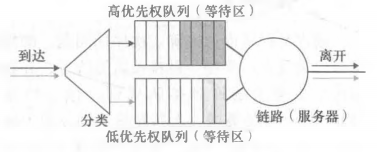
\includegraphics[width=0.6\textwidth]{image/chapter04/优先权排队模型.png}
    \caption{优先权排队模型}
\end{figure}

    每个优先权类通常都有自己的队列。当选择一个分组传输时,优先权排队规则将从队列为非空(也就是有分组等待传输)的最高优先权类中传输一个分组。在同一优先权类的分组之间的选择通常以FIFO方式完成

    下图描述了有两个优先权类的一个优先权队列的操作。分组1、3和4属于高优先权类,分组2和5属于低优先权类。

    在非抢占式优先权排队(non-preemptive priority queuing)规则下,一旦分组开始传输,就不能打断

\begin{figure}[!htbp]
    \centering
    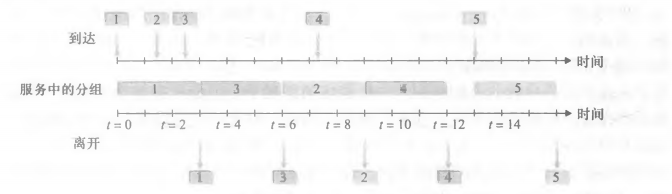
\includegraphics[width=0.8\textwidth]{image/chapter04/优先队列的操作.png}
    \caption{优先权队列的操作}
\end{figure}

\subsubsection{循环和加权公平排队}

    在循环排队规则(round robin queuing discipline)下,分组像使用优先权排队那样被分类。一个所谓的保持工作排队(work-conserving queuing)规则在有(任何类的)分组排队等待传输时,不允许链路保持空闲。当寻找给定类的分组但是没有找到时,保持工作的循环规则将立即检查循环序列中的下一个类

    下图描述了一个两类循环队列的操作。在这个例子中,分组1、2和4属于第一类, 分组3和5属于第二类。

\begin{figure}[!htbp]
    \centering
    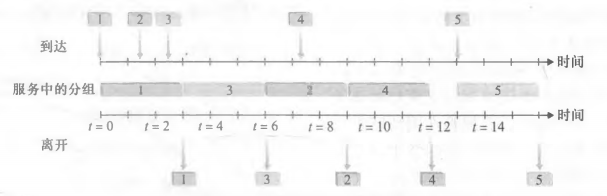
\includegraphics[width=0.6\textwidth]{image/chapter04/两类循环队列的操作.png}
    \caption{两类循环队列的操作}
\end{figure}

    一种通用形式的循环排队已经广泛地实现在路由器中,它就是所谓的加权公平排队(Weighted Fair Queuing, WFQ)规则

\begin{figure}[!htbp]
    \centering
    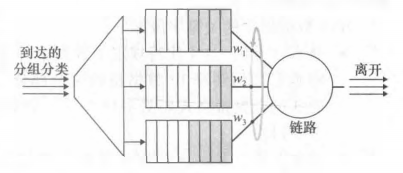
\includegraphics[width=0.6\textwidth]{image/chapter04/加权公平排队.png}
    \caption{加权公平排队}
\end{figure}

    WFQ和循环排队的不同之处在于,每个类在任何时间间隔内可能收到不同数量的服务。具体而言,每个类i被分配一个权$w_{i}$。

\section{网络协议: IPv4、寻址、IPv6及其他}

\subsection{IPv4数据报格式}

\begin{figure}[!htbp]
    \centering
    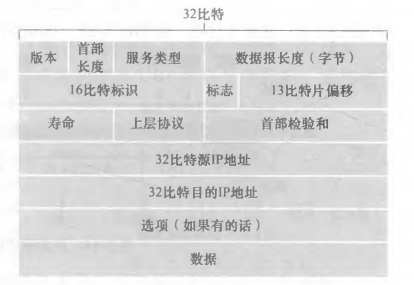
\includegraphics[width=0.6\textwidth]{image/chapter04/IPv4数据包格式.png}
    \caption{IPv4数据报格式}
\end{figure}

    IPv4数据报中的关键字段如下:

\begin{itemize}
    \item 版本号
    \subitem 这4比特规定了数据报的IP协议版本。通过查看版本号,路由器能够确定如何解释IP数据报的剩余部分。不同的IP版本使用不同的数据报格式。
    \item 首部长度
    \subitem 来确定1P数据报中载荷实际开始的地方。大多数IP数据报不包含选项, 所以一般的IP数据报具有20字节的首部
    \item 服务类型
    \subitem 服务类型(TOS)比特包含在IPv4首部中,以便使不同类型的IP数据报能相互区别开来
    \item 数据报长度
    \subitem 这是IP数据报的总长度(首部加上数据),以字节计。该长度使得IP数据报能容纳最大长度以太网帧的载荷字段
    \item 标识、标志、片偏移
    \subitem 这三个字段与所谓IP分片有关
    \item 寿命(TTL)
    \subitem 寿命(Time To Live, TTL)字段用来确保数据报不会永远(如由于长时间的路由选择环路)在网络中循环。每当一台路由器处理数据报时,该字段的值减1。若TTL字段减为0,则该数据报必须丢弃。
    \item 协议
    \subitem 该字段通常仅当一个IP数据报到达其最终目的地时才会有用。该字段值指示了IP数据报的数据部分应交给哪个特定的运输层协议
    \item 首部检验和
    \subitem 首部检验和用于帮助路由器检测收到的IP数据报中的比特错误
    \item 源和目的IP地址
    \subitem 当某源生成一个数据报时,它在源IP字段中插入它的IP地址,在目的IP地址字段中插入其最终目的地的地址。通常源主机通过DNS查找来决定目的地址
    \item 选项
    \subitem 选项字段允许IP首部被扩展。首部选项意味着很少使用,因此决定对每个数据报首部不包括选项字段中的信息,这样能够节约开销
    \item 数据(有效载荷)
    \subitem IP数据报中的数据字段包含要交付给目的地的运输层报文段(TCP或UDP)。然而,该数据字段也可承载其他类型的数据,如ICMP报文
\end{itemize}

\subsection{IPv4数据包分片}

    一个链路层帧能承载的最大数据量叫作最大传送单元(Maximum Transmission Unit, MTU)。

    因为每个IP数据报封装在链路层帧中从一台路由器传输到下一台路由器,故链路层协议的MTU严格地限制着IP数据报的长度。

    将IP数据报中的数据分片成两个或更多个较小的IP数据报,用单独的链路层帧封装这些较小的IP数据报,然后通过输出链路发送这些帧。每个这些较小的数据报都称为片(fragment)

    片在其到达目的地运输层以前需要重新组装。TCP与UDP的确都希望从网络层收到完整的、未分片的报文。

    当生成一个数据报时,发送主机在为该数据报设置源和目的地址的同时贴上标识号。发送主机通常将它发送的每个数据报的标识号加1。当某路由器需要对一个数据报分片时,形成的每个数据报(即片)具有初始数据报的源地址、目的地址与标识号。当目的地从同一发送主机收到一系列数据报时,它能够检查数据报的标识号以确定哪些数据报实际上是同一较大数据报的片。

    为了让目的主机绝对地相信它已收到了初始数据报的最后一个片,最后一个片的标志比特被设为0,而所有其他片的标志比特被设为1。另外,为了让目的主机确定是否丢失了一个片(且能按正确的顺序重新组装片),使用偏移字段指定该片应放在初始IP数据报的哪个位置。

\begin{figure}[!htbp]
    \centering
    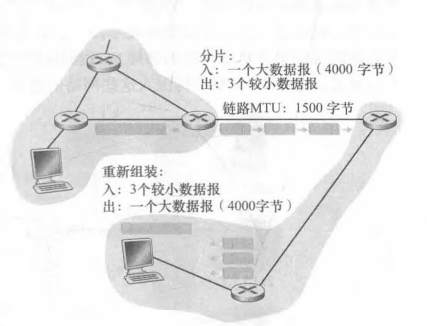
\includegraphics[width=0.6\textwidth]{image/chapter04/IP分片与重新组装.png}
    \caption{IP分片与重新组装}
\end{figure}

    一个4000字节的数据报(20字节IP首部加上3980字节IP有效载荷)到达一台路由器,且必须被转发到一条MTU为1500字节的链路上。这就意味着初始数据报中3980字节数据必须被分配为3个独立的片(其中的每个片也是一个IP数据报)

\subsection{IPv4编址}

    在讨论IP编址之前,我们需要简述一下主机与路由器连入网络的方法。一台主机通常只有一条链路连接到网络;当主机中的1P想发送一个数据报时,它就在该链路上发送。主机与物理链路之间的边界叫作接口(interface)。

    \emph{一台路由器因此有多个接口,每个接口有其链路。因为每台主机与路由器都能发送和接收IP数据报,IP要求每台主机和路由器接口拥有自己的IP地址。因此,从技术上讲,一个IP地址与一个接口相关联,而不是与包括该接口的主机或路由器相关联}。

    每个IP地址长度为32比特(等价为4字节),因此总共有$2^{32}$个(或大约40亿个)可能的IP地址。这些地址通常按所谓点分十进制记法(dotled decimal notation)书写,即地址中的每个字节用它的十进制形式书写,各字节间以句点隔开

    在全球因特网中的每台主机和路由器上的每个接口,都必须有一个全球唯一的IP地址。然而,这些地址不能随意地自由选择。一个接口的IP地址的一部分需要由其连接的子网来决定。

    下图提供了一个IP编址与接口的例子

\begin{figure}[!htbp]
    \centering
    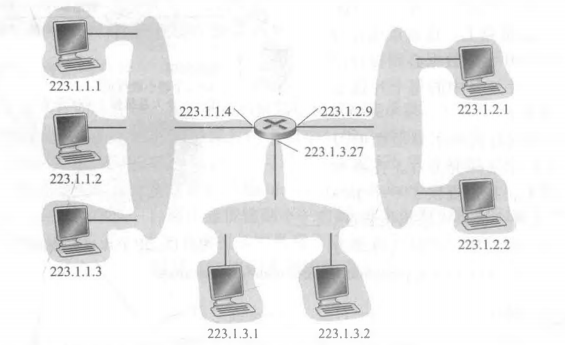
\includegraphics[width=0.6\textwidth]{image/chapter04/接口地址和子网.png}
    \caption{接口地址和子网}
\end{figure}

    左上侧的3台主机以及它们连接的路由器接口,都有一个形如223.1.1.xxx的IP地址。这就是说,在它们的IP地址中,最左侧的24比特是相同的。这4个接口也通过一个并不包含路由器的网络互联起来。该网络可能由一个以太网LAN互联,在此情况下,这些接口将通过一台以太网交换机互联

    用IP的术语来说,互联这3个主机接口与1个路由器接口的网络形成一个子网(sub-net)[RFC950]。

    IP编址为这个子网分配一个地址223.1.1.0/24,其中的/24记法,有时称为子网掩码(network mask),指示32比特中的最左侧24比特定义了子网地址。任何其他要连到223.1.1.0/24网络的主机都要求其地址具有223.1.1.xxx的形式。

\begin{figure}[!htbp]
    \centering
    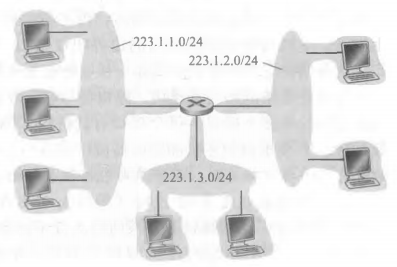
\includegraphics[width=0.6\textwidth]{image/chapter04/子网地址.png}
    \caption{子网地址}
\end{figure}

    一个子网的IP定义并不局限于连接多台主机到一个路由器接口的以太网段。

    但注意到在本例中还有其他3个子网:一个子网是223.1.9.0/24,用于连接路由器R1与R2的接口;另外一个子网是223.1.0/24, 用于连接路由器R2与R3的接口;第三个子网是223.1.7.0/24,用于连接路由器R3与R1的接口。

    对于一个路由器和主机的通用互联系统,我们能够使用下列有效方法定义系统中的子网:

    \emph{为了确定子网,分开主机和路由器的每个接口,产生几个隔离的网络岛,使用接口端接这些隔离的网络的端点。这些隔离的网络中的每一个都叫作一个子网(subnet)}

    因特网的地址分配策略被称为无类别域间路由选择(Classless Inlerdomain Routing,CIDR)[RFC 4632]。CIDR将子网寻址的概念一般化了。当使用子网寻址时,32比特的IP地址被划分为两部分,并且也具有点分十进制数形式a.h.c.d/x,其中兀指示了地址的第一部分中的比特数

    形式为a.b. c. d/x的地址的最高比特构成了 IP地址的网络部分,并且经常被称为该地址的前缀(prefix)(或网络前缀)

\subsubsection{获取一块地址}

    为了获取一块IP地址用于一个组织的子网内,某网络管理员也许首先会与他的ISP联系,该ISP可能会从已分给它的更大地址块中提供一些地址。

\begin{table*}[!htbp]
    \begin{center}
        \begin{tabular}{c c c}
            ISP的地址块 & 200.23.16.0/20 & \underline{11001000 0001011 0001}0000 00000000 \\
            组织0 & 200.23.16.0/20 & \underline{11001000 0001011 0001000}0 00000000 \\
            组织1 & 200.23.16.0/23 & \underline{11001000 0001011 0001001}0 00000000 \\
            组织2 & 200.23.18.0/23 & \underline{11001000 0001011 0001010}0 00000000 \\
            \dots\dots & \dots\dots & \dots\dots \\
            组织7 & 200.23.18.0/23 & \underline{11001000 0001011 0001111}0 00000000 \\
        \end{tabular}
    \end{center}
\end{table*}

    IP地址由因特网名字和编号分配机构(Internet Corporation for Assigned Names and Numbers,ICANN)[ICANN 2016]管理,管理规则基于[RFC 7020]。非营利的ICANN组织[NTIA 1998]的作用不仅是分配IP地址,还管理DNS根服务器。它还有一项容易引起争论的工作,即分配域名与解决域名纷争。ICANN向区域性因特网注册机构(如ARIN、RIPE、APNIC和LACNIC)分配地址,这些机构一起形成了ICANN的地址支持组织[ASOICANN 2016],处理本区域内的地址分配/管理。

\subsubsection{获取主机地址:动态主机配置协议}

    主机地址也能手动配置,但是这项任务目前更多的是使用动态主机配置协议(Dynamic Host Configuration, DHCP)[RFC 2131]来完成。

    DHCP允许主机自动获取(被分配)一个IP地址。网络管理员能够配置DHCP,以使某给定主机每次与网络连接时能得到一个相同的IP地址,或者某主机将被分配一个临时的IP地址(tempomry IP address),每次与网络连接时该地址也许是不同的。

    由于DHCP具有将主机连接进一个网络的网络相关方面的自动能力,故它又常被称为即插即用协议(plug-and-play protocol)或零配置(zeroconf)协议。

    DHCP是一个客户-服务器协议。客户通常是新到达的主机,它要获得包括自身使用的IP地址在内的网络配置信息。

\begin{figure}[!htbp]
    \centering
    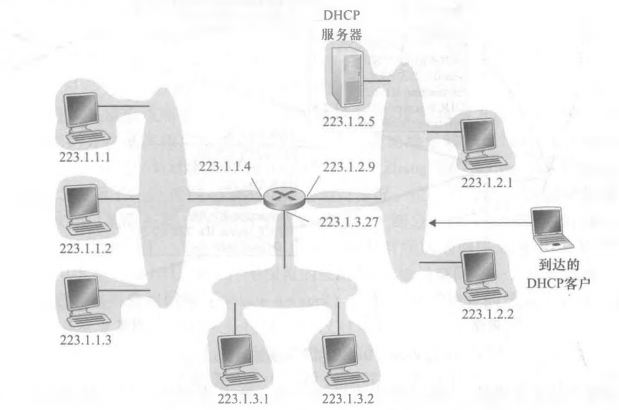
\includegraphics[width=0.6\textwidth]{image/chapter04/DHCP服务器.png}
    \caption{DHCP客户与服务器}
\end{figure}

    对于一台新到达的主机而言,针对上图所示的网络设置,DHCP协议是一个4个步骤的过程,如下图中所示。在这幅图中,yiddr(表示“你的因特网地址”之意)指示分配给该新到达客户的地址

\begin{figure}[!htbp]
    \centering
    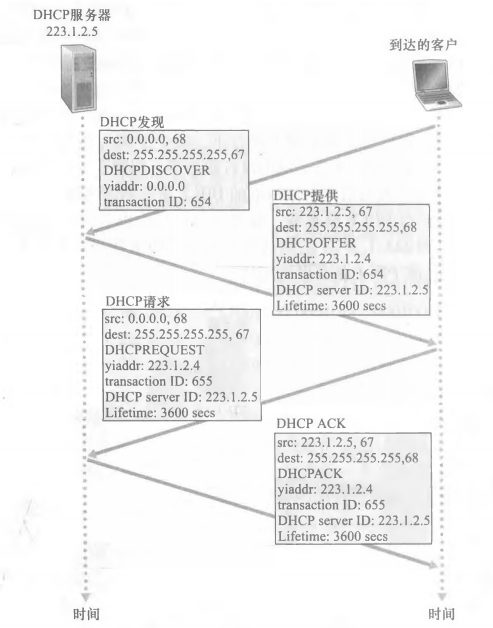
\includegraphics[width=0.4\textwidth]{image/chapter04/DHCP客户-服务器交互.png}
    \caption{DHCP客户-服务器交互}
\end{figure}

\begin{itemize}
    \item DHCP服务器发现    
    \subitem 一台新到达的主机的首要任务是发现一个要与其交互的DHCP服务器。DHCP发现报文(DHCP discover message)
    \subitem DHCP客户生成包含DHCP发现报文的IP数据报,其中使用广播目的地址255.255.255.255并且使用“本主机”源IP地址0.0.0.0。DHCP客户将该IP数据报传递给链路层,链路层然后将该帧广播到所有与该子网连接的节点
    \item DHCP服务器提供
    \subitem DHCP服务器收到一个DHCP发现报文时,用DHCP提供报文(DHCP offer message)向客户做出响应,该报文向该子网的所有节点广播,仍然使用IP广播地址255.255.255.255
    \subitem 每台服务器提供的报文包含有收到的发现报文的事务ID、向客户推荐的IP地址、网络掩码以及IP地址租用期(address lease time) , 即IP地址有效的时间量。
    \item DHCP请求
    \subitem 新到达的客户从一个或多个服务器提供中选择一个,并向选中的服务器提供用DHCP请求报文(DHCP request message)进行响应,回显配置的参数
    \item DHCP ACK
    \subitem 服务器用 DHCP ACK 报文(DHCP ACK message)对DHCP请求报文进行响应,证实所要求的参数
\end{itemize}

    \emph{从移动性角度看,DHCP确实有非常严重的缺陷。因为每当节点连到一个新子网,要从DHCP得到一个新的IP地址,当一个移动节点在子网之间移动时,就不能维持与远程应用之间的TCP连接。}

\subsection{网络地址转换}

    下次一定

\subsection{IPv6}

    由于新的子网和IP节点以惊人的增长率连到因特网上(并被分配唯一的IP地址),32比特的IP地址空间即将用尽。为了应对这种对大IP地址空间的需求,开发了一种新的IP协议,即IPv6。

\subsubsection{IPv6数据报格式}

\begin{figure}[!htbp]
    \centering
    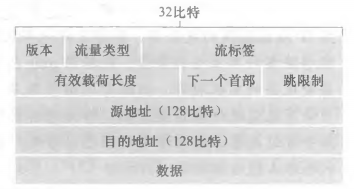
\includegraphics[width=0.6\textwidth]{image/chapter04/IPv6数据报格式.png}
    \caption{IPv6数据报格式}
\end{figure}

\begin{itemize}
    \item 扩大的地址容量
    \subitem IPv6将IP地址长度从32比特增加到128比特。
    \subitem 除了单播与多播地址以外,IPv6还引入了一种称为任播地址(anycast address)的新型地址,这种地址可以使数据报交付给一组主机中的任意一个。
    \item 简化高效的40字节首部
    \item 流标签
    \subitem IPv6有一个难以捉摸的流(flow)定义。[RFC 2460]中描述道,该字段可用于“给属于特殊流的分组加上标签,这些特殊流是发送方要求进行特殊处理的流,如一种非默认服务质量或需要实时服务的流”
\end{itemize}

